\chapter{LFT: Computer Implementation}\label{ch:MCMC}

As discussed in \secref{sec:finitetemp}, expectation values of 
physical observables $X$ in pure $\SU(2)$ LGT
are given by functional integrals
\begin{equation}\label{eq:exobs}
  \ev{X}=\frac{1}{Z}\int\DD{U}e^{-S(U)}X(U).
\end{equation}
Even though the integral~\eqref{eq:exobs} is well-defined on a lattice
because there are 
finitely many sites, it is not feasible to evaluate it numerically; even
relatively small lattices have $4\times10^4$ links. The goal of our
simulation is to estimate $\ev{X}$ by randomly generating configurations,
distributed with probability $e^{-S}$,
and on each configuration, making a measurement $X_i$. The average 
\begin{equation}\label{eq:arithmeticaverage}
  \bar{X}=\frac{1}{\nconf}\sum_{i=1}^{\nconf} X_i
\end{equation}
serves as the estimator.

The strategy of carrying out a statistical computation using random sampling
goes under the name of {\it Monte Carlo}\index{Monte Carlo} 
algorithms\footnote{The idea of Monte Carlo algorithms dates back to the 1940s.
Stanislav Ulam wanted to know the probability of winning a game of Solitaire.
The calculation turned out to be too complicated to do by hand, so he wanted to
estimate this by playing repeated games, then calculating
$$
{\rm win\ chance}\approx\frac{\rm number\ of\ wins}{\rm number\ of\ games}.
$$
Of course this is tremendously tedious; it is much more appropriate for a
computer. Other scientists working with him at Los Alamos such as John von
Neumann and Nicholas Metropolis are early pioneers of this method.}.
The strategy of drawing these random configurations is to use a
Markov chain, and hence the backbone of a lattice calculation is
often referred to as {\it Markov chain Monte Carlo} (MCMC).
Further details on MCMC methods can be found in, for instance, 
Ref.~\cite{berg_markov_2004,gattringer_quantum_2010}. 


\section{Markov chain Monte Carlo}\label{sec:MCMCintro}

To generate our configurations, we start from some arbitrary configuration
$C_0$ and construct a stochastic sequence of configurations. 
Configuration $C_i$ is generated based on\index{update}
configuration $C_{i-1}$, which we call an {\it update} or {\it Markov
step}
The result is a {\it Markov chain}
\begin{equation}
  C_0\to C_1\to C_2\to...
\end{equation}
of configurations. 

\index{MCMC}
{\it Markov chain Monte Carlo} (MCMC) is characterized by the probability 
$W^{CC'}\equiv\pr{C'|C}$, the probability to jump to configuration 
$C'$ given that the system started in configuration $C$.
The MCMC {\it transition matrix}\index{transition matrix}
\begin{equation}
  W\equiv\Big(W^{CC'}\Big)
\end{equation}
is constructed to bring the system to {\it equilibrium}.
In equilibrium, the chain should have no sinks or sources of probability,
which means that the probability of jumping into a configuration $C'$
should be the same as jumping out of $C'$. This property
is called {\it balance}\index{balance}
\begin{equation}\label{eq:balance}
    \sum\limits_CW^{CC'}\pr{C}=
    \sum\limits_CW^{C'C}\pr{C'},
\end{equation}
with the LHS representing the total probability to end up in $C'$ and
the RHS representing the probability to transition out of $C'$.
If $W$ satisfies
\begin{enumerate}
  \item {\it ergodicity},\index{ergodic} i.e.
        \begin{equation}\label{eq:ergodicity}
          \pr{C}>0\;\;\text{and}\;\;\pr{C'}>0\;\;\Rightarrow\;\;
          \exists\;n\in\N\;\;\text{s.t.}\;\;\big(W^n\big)^{CC'}>0,
        \end{equation}
        which means that every possible configuration is accessible from
        any other configuration in a finite number\footnote{In practice,
        it's important that $n$ is not too large, otherwise some configurations
        will be sampled poorly. In a sense, this is the problem with
        topological freezing\index{topological!freezing}
        in \secref{sec:toplat}.} of Markov steps;
  \item {\it normalization},\index{normalization} i.e.
        \begin{equation}
          \sum\limits_{C'}W^{CC'}=1,
        \end{equation}
        which means that starting from configuration $C$ you have
        to move somewhere;
  \item and balance, 
\end{enumerate}
then the Markov process is guaranteed to bring the ensemble toward 
equilibrium. Using normalization, one finds from \equatref{eq:balance}
\begin{equation}\label{eq:eigenProb}
    \sum\limits_CW^{CC'}\pr{C}=\pr{C'},
\end{equation}
which shows that the equilibrium distribution is a fixed point of
the Markov chain\footnote{Above, we called $W^{CC'}$ a transition matrix.
Equation~\eqref{eq:eigenProb} shows that we can think of the equilibrium
distribution as an eigenvector of $W$ with eigenvalue 1. Each component
of this vector thus yields the probability of a particular configuration.}. 


\subsection{Update: Metropolis and heat bath}
\index{heat bath}\index{Metropolis algorithm}
In this and the following subsection,
we omit the Lorentz index and space-time point from link variables to
avoid clutter.  We use $U$ to indicate the link to be updated, 
$U^\sqcup$ to indicate the staple matrix attached to $U$, and
$U'$ to indicate a trial link. We will use the Boltzmann
distribution $\pr{C}\propto e^{-S_C}$.

One trivial way to satisfy the balance condition~\eqref{eq:balance} is
to find an update that satisfies it term-by-term. For such an update, 
\begin{equation}\label{eq:detailedbalance}\index{detailed balance}
    W^{CC'}\pr{C}=W^{C'C}\pr{C'}.
\end{equation}
This property is known as {\it detailed balance}.
One of the most well-known Monte Carlo updates that satisfies detailed
balance is the {\it Metropolis algorithm}~\cite{metropolis_equation_1953}. 
In the Metropolis algorithm, a trial configuration $C'$ is selected 
with some probability distribution $\prt{C'|C}$. Then $C'$
is accepted with likelihood
\begin{equation}\label{eq:metupdate}
  \pr{C\to C'}=\min\left[1,\frac{\prt{C|C'}e^{-S_{C'}}}
    {\prt{C'|C}e^{-S_C}}\right],
\end{equation}
where $S_C$ is the action corresponding to $C$. 
If $C'$ is rejected, the unchanged configuration is counted
in the Markov chain. Using the fact that the total probability
to transition from $C$ to $C'$ is $W^{CC'}=\prt{C'|C}\pr{C\to C'}$, one
can show that this update satisfies detailed balance.

The Metropolis algorithm is in some sense the most standard Markov chain
algorithm used in lattice calculations, with the acceptance step
\equatref{eq:metupdate} being the most crucial part, in the sense that
it guarantees your configuration is drawn with the correct probability.
A Markov algorithm that concludes with the acceptance step is
said to be an\index{exact algorithm} {\it exact algorithm}\footnote{One
could imagine update steps that may not be guaranteed to draw configurations
from the desired distribution. This can be corrected by simply adding
the acceptance step at the end, and the algorithm is still exact.
One may neglect this acceptance step at the end, if one has reason to
believe the configuration is still drawn appropriately, but in such
instances the algorithm is not exact anymore.}.

Another update is the {\it heat bath} (HB). In our
simulations, a new configuration is generated from an old one by updating one
link. For the $\SU(2)$ HB algorithm, the trial link distribution is
\begin{equation}\label{eq:PTdist}
  \dd{\prt{U'}}\propto \dd U'\exp\left(\frac{\beta}{2}\,\tr\,
  U'U^\sqcup\right)
\end{equation}
and the transition probability is
\begin{equation}
  \pr{C\to C'}=\min\left[1,e^{-(S_{C'}-S_C)}\right].
\end{equation}
This construction also satisfies detailed balance. The new configuration 
is automatically accepted whenever it lowers the action, and
increases in the action are exponentially suppressed.
HB updates ensure local equilibrium, but they often 
take more CPU time. For $\SU(2)$ the guarantee of local equilibrium
turns out to be more impactful, so heat bath updates are more efficient
than general Metropolis updates.

Single link Metropolis or HB updates of links carried out in a systematic 
(as opposed to random) order fulfill balance, but do not
fulfill detailed balance.

\subsection{Update: Over-relaxation}\index{over-relaxation}

An additional useful update for $\SU(2)$ is the 
{\it over-relaxation}\index{over-relaxation} (OR) update. 
Adler introduced OR algorithms \cite{adler_over-relaxation_1981} and 
they were further developed by Creutz \cite{creutz_overrelaxation_1987} 
and others. The idea of the OR algorithm is to speed up relaxation 
by generating a group element ``far away" from $U$ without
destroying equilibrium, which is here achieved by keeping the action constant.

More precisely let $U\in\SU(N_c)$ and suppose we have some method of
choosing another link variable $U_0$ that maximizes
the action for this staple.  We assume that this method of selection has no
dependence on $U$.  Pick some element $V\in\SU(N_c)$ such that $U=VU_0$; viewed
in this way, $U$ is ``on one side of $U_0$," and the element 
``on the other side" is $U'=V^{-1}U_0$.  Note that
\begin{equation}
  V=U U_0^{-1},
\end{equation}
which implies
\begin{equation}
  U' = U_0 U^{-1} U_0.
\end{equation}
This manner of constructing a new link variable $U'$, which generates
a group element ``far away" from $U$ without changing the action, 
is what we mean by over-relaxation.

In principle an OR update should be more efficient than a Monte
Carlo update. This is because we chose the new link variable to be two
group elements away from the old one, thrusting us further
along configuration space. However unlike Metropolis updates, OR updates 
only sample the subspace of constant action, and are therefore not ergodic. 
Hence to ensure an approach to equilibrium, they must be supplemented with, 
for instance, HB updates.

We implement the $\SU(2)$ OR update by
\begin{equation}\label{eq:ORupdate}
  U\to U'=\frac{1}{\det U^\sqcup}\left(U^\sqcup UU^\sqcup\right)^\dagger.
\end{equation}
\begin{proposition}{}{OR}\label{prp:OR}
  This update does not change the $\SU(2)$ Wilson action.
  \begin{proof}
   Since $\det(kA)=k^n\det A$ for any constant $k$ and $n\times n$ matrix $A$,
   one can show that the sum of two $\SU(2)$ matrices is proportional
   to an $\SU(2)$ matrix. Hence we can write
    $$
      U^\sqcup=u^\sqcup\sqrt{\det U^\sqcup}
    $$
    where $u^\sqcup\in\SU(2)$. After updating, the local contribution
    to the Wilson action becomes
    \begin{equation*}
      \tr U'U^\sqcup =\frac{1}{\det U^\sqcup}\tr
                       \left(U^\sqcup UU^\sqcup\right)^\dagger
                     =\tr U^\sqcup U\left(u^\sqcup\right)^\dagger u^\sqcup
                     =\tr U^\sqcup U,
    \end{equation*}
    which is what it was originally.
  \end{proof}
\end{proposition}
Since the action is unchanged, the proposal is always accepted. This simple 
behavior is special to $\U(1)$ and $\SU(2)$ LGT. Its usefulness is 
extended to $\SU(N_c)$ when $N_c>2$ via the method of Cabibbo and Marinari
\cite{cabibbo_new_1982}.

\subsection{Update: Over-relaxation gauge fixing}\label{sec:ORgaugefix}

\index{gauge!fixing}
In general expectation values of gauge-dependent quantities are zero.
Nevertheless there are some rare occasions where it is useful to calculate
a quantity in a particular gauge, which can then be related to some
other physical quantity. In this section we cover an OR
algorithm that fixes gauge configurations to the {\it Coulomb} or 
{\it Landau} gauges.\index{gauge!Coulomb}\index{gauge!Landau}
In the continuum such gauges are given by the condition
\begin{equation}
  \partial_\mu A_\mu=0,
\end{equation}
where $\mu$ runs over only spatial directions for the Coulomb gauge, and
over all four directions for the Lorentz gauge. On the lattice, these 
{\it gauge conditions}\index{gauge!condition} are discretized as
\begin{equation}
  \Delta(x)\equiv A_\mu(x)-A_\mu(x-a\hat\mu) =0.
\end{equation}

\begin{proposition}{}{ORgf}
A gauge satisfying $\Delta(x)=0$ is achieved by extremizing
$$
  F\equiv-\Re\tr\sum_{x,\mu} g(x) U_\mu(x) g^\dagger(x+a\hat{\mu})
$$
\begin{proof}
Any gauge matrix can be written
$$
  g=e^{is^aT^a},
$$
where $s^a\in\R$ and $T^a$ are the generators of the Lie group. We want
to find the special $g_0$ that extremizes $F$; this is equivalent to finding
the $s_0$ that extremizes it. We will look in the vicinity of such a
gauge, i.e. look at gauges 
$$e^{i\tau^a T^a}, \qquad\tau\equiv s-s_0$$
with $\tau$ small. Then
\begin{equation*}\begin{aligned}
  F&=-\Re\tr\sum_{x,\mu}&&
      e^{i\tau^a(x)T^a}\,e^{iaA^b_\mu(x)T^b}\,e^{-i\tau^c(x+a\hat\mu)T^c}\\
   &\approx &&\big(\id+i\tau^a(x)T^a\big)
        \big(\id+iaA_\mu^b(x)T^b\big)
        \big(\id-i\tau^c(x+a\hat\mu)T^c\big)\\
   &\approx && \big(\id+a\tau^c(x+a\hat\mu)A_\mu^b(x)T^bT^c
                       -a\tau^a(x)A_\mu^b(x)T^aT^b\big),
\end{aligned}\end{equation*} 
where we have neglected $\order{a^2, a\tau, \tau^2}$ terms and use that
the $T^a$ are traceless. At the extremum, derivatives with respect to $\tau$
will vanish. Exchanging our dummy group summation indices and shifting
the first term by one site (which is allowed because of 
periodic BCs) we find
\begin{equation*}\begin{aligned}
  0=\pdv{F}{\tau^d}
     &=-\Re\tr\sum_{x,\mu}&&a\pdv{\tau^d}
        \left[A_\mu^b(x-a\hat\mu)\tau^c(x)-A_\mu^b(x)\tau^c(x)\right]T^bT^c\\
     &= &&a\left[A_\mu^b(x-a\hat\mu)-A_\mu^b(x)\right]T^bT^d.
\end{aligned}\end{equation*}
In order for the above to vanish, the term in brackets has to vanish,
which completes the proof.
\end{proof}
\end{proposition}
The strategy from here is to minimize $F$. As you can clearly see from
its definition, this can be accomplished through the replacement
\begin{equation}\label{eq:gfORupdate}
U\to U'=gU_\mu g^\dagger,
\end{equation}
which is reminiscent of the OR update~\eqref{eq:ORupdate}. Hence we employ
again OR, i.e. we find the $g$ minimizing $F$ and make the
replacement~\eqref{eq:gfORupdate}. In a similar strategy as
\propref{prp:OR}, we look at the local update to $F$,
\begin{equation}
  \Re\tr g(x)\sum_\mu\left[U_\mu(x)g^\dagger(x+a\hat\mu)
                        +U_\mu^\dagger(x-a\hat\mu)g^\dagger(x-a\hat\mu)\right]
  \equiv\Re\tr g(x)K(x).
\end{equation}
As before, $K(x)=\sqrt{\det K(x)}\hat K(x)$, where $\hat K(x)\in\SU(2)$.
To extremize $F$, we search for the $g$ rotating everything under the
trace to $\id$, which is clearly
\begin{equation}
  g(x)=K^\dagger(x)/\sqrt{\det K(x)}.
\end{equation} 

We will never achieve the condition $\Delta(x)=0$ on the computer exactly.
A measure of how close we are to satisfying the gauge condition is
\begin{equation}
  \theta\equiv\frac{1}{N_c N_s^3}\sum_x\tr\Delta(x)\Delta^\dagger(x).
\end{equation}
This combination is constructed so that $\theta\in\R$. 

For more information
about using OR to gauge fix, see Ref.~\cite{mandula_efficient_1990}. 
For information about how to implement this on multiple GPUs, see
e.g. Ref.~\cite{schrock_coulomb_2013}.

\subsection{Choosing a random number generator}

As far as we know\footnote{See for instance \apref{ap:bell}.}, 
the only truly random or stochastic things in nature are
quantum mechanical measurements. This poses a problem for our strategy, since
we need a random number for the Metropolis step \equatref{eq:metupdate}.
In practice, one wants to generate a number $X$ uniformly at random
in the interval $X\in[0,1)$ and compute the number on the RHS
of \equatref{eq:metupdate}. If $X$ turns out to be greater, you reject $C'$.

In order to generate $X$, we use a {\it random number
generator}\index{generator!random number} or RNG. 
Since we can't have a true random number\footnote{For
this reason, these algorithms are sometimes more aptly called
{\it pseudorandom number generators}\index{generator!pseudorandom number}
or PRNGs.}, we instead settle for an algorithm that produces a sequence of numbers
\begin{equation}
  X_{\rm seed},~X_1,~X_2,~...,~X_n,~...,
\end{equation}
by using some rule to generate $X_{n+1}$ given $X_n$. The starting number is
called the {\it seed}\index{seed}. The goal is to choose your rule so that,
given the seed, it is difficult or effectively impossible to figure out what
$X_n$ will be. Again, this is not a truly random process, but unfortunately it
is not yet practical to harness direct quantum-mechanical measurements to that
end. 

One of the earliest popular RNGs was the {\it linear congruence
generator}\index{generator!linear congruence}~\cite{lehmer_mathematical_1951,thomson_modified_1958}. 
Here the rule is pretty simple
to understand: You choose three tuning parameters $a$, $b$, $m\in\N$
and then generate according to
\begin{equation}\label{eq:linearCongruence}
X_{n+1}=(aX_n+b)\mod m.
\end{equation}
One can then convert a number $X_n$ generated in this way to a number $X$
in the unit interval as required for the Metropolis step by normalizing it by $m$.


\begin{figure}
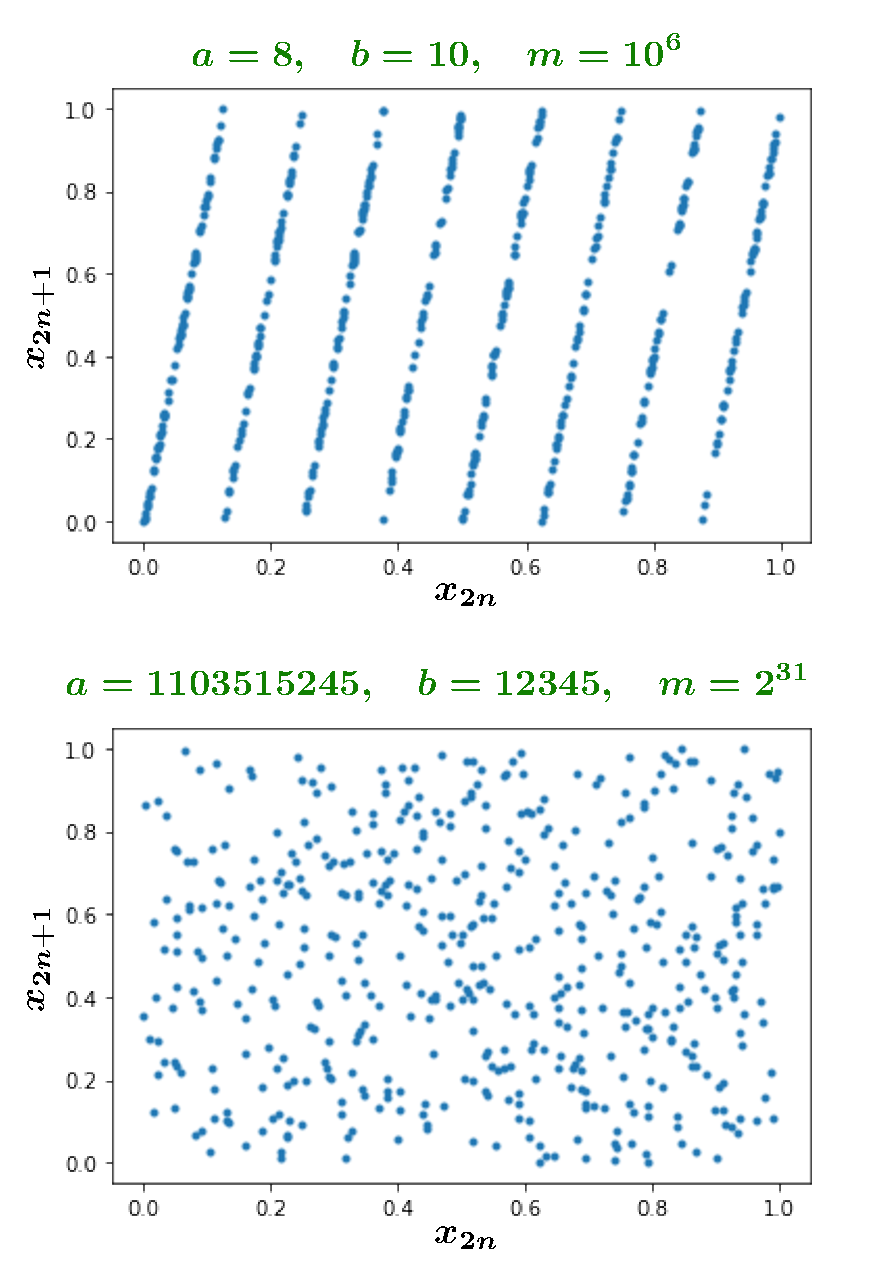
\includegraphics[width=\linewidth]{figs/linear_congruence.pdf}
\caption{A strong correlation hidden in the linear congruence generator for
poorly chosen $a$, $b$, and $m$. Things seem to improve for a better choice of
these parameters, but as Marsaglia proved, this generator ought to be avoided
regardless. Image made by C. Schmidt.}
\label{fig:LCG}
\end{figure}

The linear congruence generator is extremely easy to implement and is quite
fast. Unfortunately it suffers from one fatal flaw: It sucks. To see that it
sucks, one can plot $X_{2m}$ against $X_n$. An example of such a plot for
poorly chosen $a$, $b$, and $m$ is given in \figref{fig:LCG}. One sees the
pairs organize themselves into planes. Changing $a$, $b$, and $m$ seems
to improve the generator, but this flaw of the linear congruence generator
is fundamental. Indeed it was shown by Marsaglia~\cite{marsaglia_random_1968} that
outcomes of the linear will always arrange themselves in planes of hypercubes.
Hence one should never this generator for scientific purposes.

Looking for these hidden correlations is a bit challenging requiring some care
and experience. There are a variety of tests, but if you want to be thorough,
it is likely best to use already existing batteries, such as the {\it Diehard}
battery written by Marsaglia himself. More modern batteries, 
such as the {\it Dieharder}, can be found online~\cite{dieharder}.
Besides lacking hidden correlations, you would like numbers produced by your
RNG to match the target distribution. This can be quantitatively estimated
using, for instance, the Kolmogorov test of \secref{sec:kolm}.
Some modern RNGs that are known to be suitable for scientific purposes,
in particular passing some of the tests above, include
the\index{generator!Tausworthe} 
{\it hybrid Tausworthe}~\cite{tausworthe_random_1965,lecuyer_maximally_1996}
and\index{generator!Mersenne twister} 
the {\it Mersenne twister}~\cite{matsumoto_mersenne_1998}.

\section{Statistical analysis}\label{sec:statana}

Since $C_i$ is generated based on $C_{i-1}$, measurements on subsequent
configurations are correlated. In our simulations, these
correlations are reduced in two ways:
\begin{enumerate}
  \item Subsequent configurations are separated by multiple updating sweeps;
        and then
  \item configurations are grouped into $\nconf$ blocks or bins.
\end{enumerate}
The final measurements $X_i$ used in data analysis are obtained by averaging
within each block.
To check whether the final data are effectively independent, one can use
the integrated autocorrelation time. 
For statistically independent measurements, we expect the variance 
$\sigma^2_{\bar{X}}$ of $\bar{X}$ to be
\begin{equation}
  \sigma^2_{\bar{X}}=\frac{\sigma^2}{\nconf}
\end{equation}
due to the CLT. In practice, however, one finds 
\begin{equation}
  \sigma^2_{\bar{X}}=\frac{\sigma^2}{\nconf}\tauint.
\end{equation}\index{autocorrelation time!integrated}
The factor $\tauint$ is the integrated autocorrelation time. It is the 
ratio between the estimated variance of the sample
mean and what this variance would have been if the data were independent.
For effectively independent data, $\tauint=1$.

So, the final measurements are drawn from some
distribution with mean $\ev{X}$ and variance $\sigma^2$
and are effectively independent. The
estimator $\bar{X}$ of the mean is the average~\eqref{eq:arithmeticaverage}, 
while the unbiased estimator $\bar{\sigma}^2$ of the variance is
\begin{equation}\label{eq:estimatorvariance}
  \bar{\sigma}^2=\frac{1}{\nconf-1}\sum_{i=1}^{\nconf}
      \left(X_i-\bar{X}\right)^2.
\end{equation}
An estimator is biased if its mean for finite $\nconf$ 
does not agree with the exact result;
the bias is the difference. Generally, problems with bias emerge whenever
one wishes to estimate some non-linear function $f$ of the mean $\ev{X}$.
Naively one might guess
\begin{equation}
  \bar{f}_\text{bad}=\frac{1}{\nconf}\sum_{i=1}^{\nconf}f(X_i)
\end{equation}
as an estimator; however $\bar{f}_\text{bad}$ is not guaranteed
to converge to the exact result\footnote{See for instance the discussion
in \secref{sec:bias}.}. 
An estimator for $f(\ev{X})$ that converges to its true value is
\begin{equation}\label{eq:MCMCconsistentEst}
  \bar{f}=f(\bar{X});
\end{equation}
in particular, the bias of this estimator is $\order{1/\nconf}$.
Therefore in the large $\nconf$ limit, the bias vanishes faster than the 
statistical error bar.

At this point it is worth commenting when it is appropriate to use
the sample average~\eqref{eq:arithmeticaverage} and the estimator
\eqref{eq:MCMCconsistentEst}. The sample average is the preferred 
method to estimate an observable that can be directly calculated from 
the configurations, i.e. when $X_i=X(C_i)$. 
Such random variables are called {\it primary quantities},
\index{primary quantity} and they include many simple observables such
as the action, the absolute value of the Polyakov loop, and so on. 
However some quantities can only be calculated 
as functions of the sample average; these are called {\it secondary quantities}.
\index{secondary quantity} An obvious example is the variance, which is defined
only in terms of averages. But a less obvious example are particle masses,
which cannot be directly calculated on any single configuration. In this
case we are forced to use \equatref{eq:MCMCconsistentEst}.

We have introduced a way to estimate the mean and variance of some
operator, as well as a way to estimate the mean of some function of
that operator. Now we need a way to estimate the error bar of that
function. We cannot use
\begin{equation}
  \bar{\sigma}^2_{\bar{f}}=\frac{\bar{\sigma}^2_{\bar{f}}}{\nconf}
    =\frac{1}{\nconf\,(\nconf-1)}\sum_{i=1}^{\nconf}
     \left(f(X_i)-\bar{f}\right)^2
\end{equation}
because $f(X_i)$ is not a valid sample point.
One could analytically produce an error bar for $\bar{f}$ 
using error propagation. However when the function is complicated, 
error propagation becomes extremely unwieldy.

Jackknifing\index{jackknife} allows one to extract a mean and error bar,
and it is straightforward to implement; 
therefore it makes sense to use the jackknife method generally.
The idea of jackknifing is to throw away the first measurement, 
leaving $\nconf-1$ resampled values. Then we resample again, this
time throwing out the second point, and so on. The resulting
jackknife bins are
\begin{equation}
  X_{J,i}=\frac{1}{\nconf-1}\sum_{j\neq i}X_j.
\end{equation}
The jackknife estimator for $f(\ev{x})$ is then
\begin{equation}
  \bar{f}_J=\frac{1}{\nconf}\sum_{i=1}^{\nconf}f(X_{J,i}),
\end{equation}
while the estimator for the variance of $\bar{f}_J$ is
\begin{equation}
  \bar{\sigma}^2_{f_J}=\frac{\nconf-1}{\nconf}\sum_{i=1}^{\nconf}
    \left(f(X_{J,i})-\bar{f}_J\right)^2.
\end{equation}

In many instances, we will need to compare two estimates 
of the same quantity against each other and decide whether the difference 
between them is significant. This can happen, for example, if we want to
compare another group's results with our own. Let their result
be $\bar{X}$ with uncertainty $\sigma_{\bar{X}}$ and ours be
$\bar{Y}$ with uncertainty $\sigma_{\bar{Y}}$. Then the probability
that these two estimates differ by at least $D$ is
\begin{equation}\index{Gaussian difference test}
  q=\pr{|\bar{X}-\bar{Y}|>D}
    =1-\erf\left(\frac{D}{\sqrt{2
     \left(\sigma_{\bar{X}}^2+\sigma_{\bar{Y}}^2\right)}}\right)
\end{equation}
assuming $\bar{X}$ and $\bar{Y}$ are normally distributed with
the same mean. This is called a Gaussian difference test. 
The quantity $q$ is called the q-value.
In practice we take $q\leq0.05$ to be an indication of a possible 
discrepancy between $\bar{X}$ and $\bar{Y}$, keeping in mind that 
$q\leq0.05$ by chance one out of twenty times.

In practice, the true variances $\sigma_{\bar{X}}$ and $\sigma_{\bar{Y}}$
are not known. If one wishes to use the estimators $\bar{\sigma}_{\bar{X}}$
and $\bar{\sigma}_{\bar{Y}}$ instead, one can perform a {\it Student
difference test} or {\it t-test}\index{t-test} to investigate whether the 
discrepancy $D$ is due to chance. Suppose the estimate $\bar{X}$ comes from 
$M_{\text{conf}}$ data, while $\bar{Y}$ comes from $\nconf$ data.
Assume $\sigma_{\bar{X}}=\sigma_{\bar{Y}}$, which
happens when the sampling methods used are identical.
We introduce the random variable
\begin{equation}
  t=\frac{D}{\bar{\sigma}_D},
\end{equation}
where $D=\bar{X}-\bar{Y}$, and
\begin{equation}
  \bar{\sigma}^2_D=\left(\frac{1}{M_{\text{conf}}}+\frac{1}{\nconf}\right)
                   \frac{(M_{\text{conf}}-1)\,\bar{\sigma}_{\bar{X}}^2
                    +(\nconf-1)\,\bar{\sigma}_{\bar{Y}}^2}
                   {M_{\text{conf}}+\nconf-2}.
\end{equation}
Then the probability that these two estimates differ by at least $D$ is
\begin{equation}
 q=2
 \begin{cases}
 \,I\left(z,\frac{\nu}{2},\frac{1}{2}\right) & \text{for }t\leq 0, \\
 \,1-\frac{1}{2}\,I\left(z,\frac{\nu}{2},\frac{1}{2}\right) & \text{otherwise},
 \end{cases}
\end{equation}
where $I$ is the incomplete beta function, $\nu=M_{\text{conf}}+\nconf-2$,
and
\begin{equation}
  z=\frac{\nu}{\nu+t^2}.
\end{equation}

To estimate finite size corrections and carry out continuum limit
extrapolations, we need a way to fit data to curves.
Consider a sample of $\nsim$ Gaussian, independent data points $(X_i,Y_i)$,
where the $Y_i$ have standard deviations $\sigma_i$ and the $X_i$ have
no errors. For instance, if one is interested in a continuum limit
extrapolation, the $X_i$ are $\beta$ values while the $Y_i$ are
ratios of scales evaluated at that $\beta$.
We model these data with a fit that depends on some set
of $M$ parameters
\begin{equation}
  y=y(x;a),
\end{equation}
where $a=(a_1,...,a_M)$ is the vector of these parameters. Our goal
is to estimate the $a_j$.
Assuming that $y(x;a)$ is the exact law for the data, the probability
distribution for the measurements $Y_i$ is 
\begin{equation}
  f(y_1,...,y_{\nsim})=\prod_{i=1}^{\nsim}\frac{1}{\sqrt{2\pi}\sigma_i}
      \exp\left[\frac{-(y_i-y(x_i;a))^2}{2\sigma_i^2}\right].
\end{equation}
The probability that the data fall within a region near what was observed is
\begin{equation}
  \text{P}=\prod_{i=1}^{\nsim}\frac{1}{\sqrt{2\pi}\sigma_i}
      \exp\left[\frac{-(y_i-y(x_i;a))^2}{2\sigma_i^2}\right]dy_i.
\end{equation}
Our strategy for determining the correct fit will be to find the vector $a$
that maximizes the above probability. This happens when
\begin{equation}
  \chi^2(a)\equiv\sum_{i=1}^{\nsim}\frac{(y_i-y(x_i;a))^2}{2\sigma_i^2}
\end{equation}
is minimized. This strategy is an example of a {\it maximum likelihood method}.

We now describe an iterative method to search for the minimum of $\chi^2$.
Let $a_n$ be the vector of parameters for the $n\nth$ iteration.
As long as $a$ is in a small enough neighborhood of $a_n$, we can safely
approximate
\begin{equation}\label{eq:NRapprox}
  \chi^2(a)\approx\chi^2(a_n)+(a-a_n)\cdot b
           +\frac{1}{2}(a-a_n)\,A\,(a-a_n),
\end{equation}
where the coefficients of the vector $b$ and the $M\times M$ matrix $A$ 
are given by the first and second derivatives of $\chi^2$ evaluated at $a_n$.
In the {\it Newton-Raphson method}\index{Newton-Raphson}, the next 
iteration $a_{n+1}$ is
determined from the condition $\nabla\chi^2(a)|_{a=a_{n+1}}=0$,
which yields
\begin{equation}\label{eq:NR}
  a_{n+1}=a_n-A^{-1}b.
\end{equation}
If the approximation~\eqref{eq:NRapprox} is not good, one can instead move
a small step in the direction of the gradient by
\begin{equation}\label{eq:SD}
  a_{n+1}=a_n-c\,b,
\end{equation}
where $c$ is a constant that is small enough not to overshoot direction
of steepest descent. This is an example of a {\it steepest descent method}.
The Levenberg-Marquardt\index{Levenberg-Marquardt} 
method~\cite{levenberg_method_1944,marquardt_algorithm_1963} 
varies smoothly between~\equatref{eq:NR} and 
\eqref{eq:SD}. Steepest descent is used far from the minimum, and 
then it switches to the Newton-Raphson method when the minimum is approached.

\section{General code structure}

Now that we have introduced the general idea of MCMC, along with some specific
updating schemes, and complications for statistical analysis, we are ready 
to discuss the computer implementation. In this section we will discuss the
general code structure. In the following sections, we will address various
implementation details important for improving code performance and readability. 


As mentioned earlier, we design the simulation using {\it local updates}, which
means we update the links one at a time. This is done in a systematic order,
because there is some computational advantage compared to updating in a
random order~\cite{berg_markov_2004}. 
An updating {\it sweep}\index{sweep} updates every link on the lattice once. 
To maximize efficiency while maintaining ergodicity, it is common for pure
$\SU(2)$ algorithms to use
a combination of HB and OR updating. 


An MCMC simulation of LGT broadly consists of three essential steps:
\begin{enumerate}
  \item {\it Initialization}: The first thing to do is get everything ready for
        the simulation. This includes initializing the random number generator,
        and setting up an initial configuration.
  \item {\it Equilibration} or {\it thermalization}:
        \index{equilibration}\index{thermalization}
        To avoid over-sampling rare configurations,
        one must perform many sweeps to bring the system to its equilibrium 
        distribution. The structure of this section looks like 
        \begin{verbatim}
        do from n=1 to n=nequi 
          call MCMC update
        end do
        \end{verbatim}
  \item {\it Configuration generation}: One we are in the equilibrium
        distribution, we want to generate configurations on which we can
        perform measurements. To help reduce correlations between
        measurements, multiple updating sweeps are performed in between.
        This section is structured as
        \begin{verbatim}
        do from n=1 to n=nconf
          do from n=1 to n=ndiscarded
            call MCMC update
          end do
          save configuration 
        end do
        \end{verbatim}
  \item {\it Measurements}: Now that we have a good sample of configuration
        space, we are ready to perform measurements there. Some measurements
        can be take {\it in situ}, i.e. they are incredibly cheap and can be
        calculated the moment the configuration is saved. Measurements of this
        type include simple link products like the Polyakov loop. More expensive
        observables may require inverting a Dirac matrix thousands of times, 
        gauge fixing, or smoothing. For such observables it is better to
        have separate code that runs on the saved configurations. This
        code is structured as
        \begin{verbatim}
        do from n=1 to n=nconf
          take measurement 
        end do
        \end{verbatim}
\end{enumerate}

\section{Object-oriented programming}\label{sec:oop}


The focus of these research notes is on LFT, which employs programming heavily.
In particular the computationally demanding MCMC code we write spurs us to
write code that is
\begin{enumerate}
  \item easy to read,
  \item well organized,
  \item future-proof, and
  \item high performance.
\end{enumerate}
Furthermore we must carry out statistical analysis of observables measured on
configurations produced by this MCMC code. In this Appendix we collect
some information on these topics.


The first programming language I used for serious scientific calculations
\index{object-oriented programming}
was Fortran. Fortran does not traditionally 
allow\footnote{Actually I think more modern Fortran compilers 
allow for OOP, but I get the impression that C++ is the preferred language
in scientific computing for this.} for object-oriented programming (OOP); 
instead, very roughly, Fortran only
allows for two things:
\begin{enumerate}
  \item arrays or variables of some kind, along with 
  \item some functions that map them into each other.
\end{enumerate}
Actually programming in Fortran is kind
of a physicist's dream: it is very direct, and you can see exactly what
operations the computer is going to carry out. I will call Fortran
a {\it non-OOP} language.

An OOP language is more general than this, and hence it is a bit more powerful.
\index{compile time}\index{run time}
For the following discussion, it is useful to introduce two terms,
{\it compile time}, which is the time during which the code you wrote
is turned into an executable, and {\it run time}, which is the time during
which the executable runs.
Again very roughly, an OOP language has instead three things:
\begin{enumerate}\index{object}\index{function!OOP}\index{method}\index{class}
  \item {\it objects}, which I will define as any runtime entity that 
        takes up memory and has an address;
  \item {\it functions} or {\it methods}, which map objects to other
        objects; and
  \item {\it classes}, which are an abstraction of objects and/or functions,
        that do not take any space in memory or have an address. One common
        way to think of classes is as ``blueprints" for objects.
\end{enumerate}

Ultimately an important goal of OOP is to try to make your code more closely
mirror how things look in the real world, and maybe you can see that this
goal is more readily accomplished under this paradigm.
For example in point (1), you can see that variables
and arrays were generalized to objects. This gives you more flexibility in
coding, in case the real-world object you are thinking of is not easily
imagined as a variable or an array. The way that we invent these objects
is through point (3), the class. In addition to defining objects, the
class is an important organizational tool, allowing you to collect all
objects and functions that are related to some general idea,
which\index{encapsulation}\index{abstraction} is sometimes called 
{\it encapsulation}. Both functions and classes
are useful to hide implementation details from the programmer, minimizing
the what the programmer needs to provide to the program, which is
sometimes called {\it abstraction}.

Encapsulation and abstraction are useful to programmers in part because
they make the code much more readable (again because what you are typing
more closely resembles how you think of things in the real world) and
reduce code duplication (which prevents you from having to maintain
several duplicates). Furthermore you
can change the implementation details of that class
without having to modify anything that utilizes it. The drawback is that
it can be difficult to see precisely what operations the computer
performs. In my experience, this trade-off is hugely worthwhile, and I think
most modern software developers would agree.


\subsection{OOP in C++} 
Probably the best way to learn is through an example. To see the basics
of OOP in action, we will implement a \texttt{CAT} class, and 
introduce some new OOP jargon and concepts along the way.
The example code definitely works for C++14~\cite{cppDocumentation},
but it likely also works for earlier standards.

The first function we define, \texttt{narrate}, is not part of the class;
actually it is there to make it easier to print to screen, which is
an example of abstraction. We see that it made the code easier to
read and reduced duplication.\\

\begin{code*}
\mycode{c++}{exampleCode/cat.cpp}
\end{code*}

The \texttt{CAT} class begins with the \texttt{public} keyword, which
is a statement about accessibility. Anything that falls under the
\texttt{public} heading can be used outside of the class\footnote{The other
two possibilities are \texttt{private} and \texttt{protected}. 
Anything under the \texttt{private} heading
can only be seen by the class itself, while \texttt{protected} members can be accessed 
by the class itself, as well as any derived classes that inherit from the class.}. 
Everything in the class falls
under this heading in this example. The first group of three lines
are variables stored inside the \texttt{CAT} class; such variables
\index{attribute}\index{constructor}\index{destructor}\index{method}
are called {\it attributes}. The next group of two functions are
the {\it constructor} and the {\it destructor}, which I will explain
shortly. Finally the last group of four \texttt{void} functions are 
called {\it methods}. It is basically correct to think of a class as a
collection of attributes and methods acting on them.\\

\begin{code*}
\mycode{c++}{exampleCode/cat.cpp}
\end{code*}

To understand the constructor and destructor, let us turn to our main
code where we will use this class. In the first line, we declare a
\texttt{CAT}-type\footnote{A {\it type}\index{type} is a category of data
defined by some properties or characteristics. The type often defines the sorts
of operations that one can do with that datum. For instance, integers, floats,
strings, and objects are all types. Types are related to classes but not exactly
the same. A class in particular tells you how something should be implemented,
whereas a type doesn't necessarily. For instance you might have a \texttt{CAT}
type. Two possible \texttt{CAT}-type implementations could be, e.g.
\texttt{MEANCAT} or \texttt{WUNKUSCAT} classes.} object, which we call \texttt{cat}. We say that we have
{\it instantiated} \texttt{cat}, and \texttt{cat} is an {\it instance}
\index{instantiation}
of \texttt{CAT}. \texttt{CAT} is a class; therefore, as mentioned
earlier, it takes up no memory and has no address associated to it.
On the other hand, \texttt{cat} is an object, and hence has some
memory associated to it at runtime. More precisely, it uses the
amount of memory required to hold its attributes.

The constructor is the function that is called every time an object is
instantiated. If you look back at the \texttt{CAT} class, you can see that
the constructor takes an argument called \texttt{name}. In the main,
the string ``Chooky" is being fed into this argument. A constructor does
not have to take an argument, or even explicitly do anything, but often
it is useful to have a constructor set the attributes to some default values.
That is what the constructor does in this case, and it also tells the
user that it instantiated a \texttt{CAT} object.\\

\begin{code*}
\mycode{text}{exampleCode/catOutput.txt}
\end{code*}

The destructor is the function called every time an object is destroyed.
The two most common times an object is destroyed are when the object
leaves scope and when the program ends. Scopes in C++ are defined by
curly brackets $\{\}$. So for example if you define a new variable
inside a function, and you only use this variable inside that function,
the {\it scope} of that variable is the inside of the function. 
Other examples of scope include
the inside of \texttt{if} and \texttt{while} statements and the
\index{scope}
insides of classes. Look to \texttt{scope.cpp} to see constructors and
destructors in action. Note the order of creation and destruction.

This practice of objects automatically allocating memory through their
constructors and destroying themselves when they leave scope
sometimes goes under the name\index{resource acquisition}
{\it resource acquisition is initialization} (RAII).
This strategy helps avoid\index{memory leak} {\it memory leaks},
which is when the computer fails to release some unneeded 
memory\footnote{Failure to release memory can negatively impact performance;
for instance if you never release memory, then long and memory-intensive
programs will quickly use up all of a system's available memory.}.

Turning back to the main, we see that we can access attributes of
\texttt{cat} such as \texttt{\_name} directly, and we can also call
methods of \texttt{cat} like \texttt{speak()}. This is possible because
we made these public attributes and methods. Note that inside the class,
it is enough to use the attribute or method name by itself. Outside the
class, i.e. inside the main, we have to use the object as an 
intermediary.

Hopefully this is enough for you to get at least an intuition for
what OOP is, how it works, and why someone would want to use it. These
few pages are just the beginning; there are many more advanced
features available to C++ that make classes extremely generalizable.
Besides the advantages of being object-oriented, C++ also has many
features that make it valuable for high-performance computing.
For example you can manipulate exactly where and how objects
are stored in memory. There are lots of good references for OOP
in C++ out there, but a good start might be Ref.~\cite{tp:cpp}.\\

\begin{code*}
\mycode{c++}{exampleCode/scope.cpp}
\end{code*}
\begin{code*}
\mycode{text}{exampleCode/scopeOutput.txt}
\end{code*}

\subsection{OOP in Python}

We continue by discussing OOP in Python. Python is a rather friendly language
and it is popular for scientific programming, so you can find lots of useful
tutorials online, for instance here~\cite{pythonOOP}. We will use
Python3~\cite{python3}.

In this section we will demonstrate
a couple other important features of the OOP paradigm. In particular we will
discuss {\it inheritance},\index{inheritance} the process by which a
class (the {\it child}\index{child} class) inherits attributes and methods
from a more general class (the {\it parent}),\index{parent} and
{\it operator overloading}, \index{operator overloading} where one generalizes 
operators such as $+$ to function with objects of the class you defined.
Inheritance is useful organizationally as it helps you think of some class
as a special case of a more general class. Furthermore it reduces code
repetition, since the child has access to all methods and attributes defined in
the parent. Operator overloading enhances readability, for example by
helping your code more closely mirror mathematical notation.\\

\begin{code*}
\mycode{python}{exampleCode/cat.py}
\end{code*}

Let us begin by implementing the \texttt{CAT} class from before in Python,
which is shown in \texttt{cat.py}. One nice feature of Python classes
is the \texttt{\_\_doc\_\_} attribute, which is set here as the first string
in quotes, giving a description of the class. Note also that Python
does not have the \texttt{private} or \texttt{public} distinction that
C++ has; indeed all attributes and methods in Python OOP are effectively 
public\footnote{You can obfuscate attributes by leading with a double 
underscore \texttt{\_\_} so that it is not as easily accessible. Still, there 
are ways to access such attributes.}.
The constructor and destructor\footnote{Python does not treat scope the same
way as C++, so an object is not destroyed automatically when you e.g.
exit a \texttt{for} loop. Automatic object destruction in Python 
happens through \index{garbage collection}
its {\it garbage collector}, for example when the program terminates,
or when an object loses its reference by being reassigned.} are identified with
\texttt{\_\_init\_\_} and \texttt{\_\_del\_\_}, respectively. All of
\texttt{\_\_init\_\_}, \texttt{\_\_del\_\_}, and \texttt{\_\_doc\_\_} 
are examples of
Python special functions, which will be discussed in a bit more detail
when we get to operator overloading. 
Two more syntactical characteristics 
to point out are that methods always take the \texttt{self}\footnote{The
\texttt{self} keyword refers to particular instance which is using
the called method.} reference as 
the first argument, and that this reference is always required to
interact with class methods and attributes, even within the class itself.
Some example output code using the \texttt{CAT} class is shown below.\\

\begin{code*}
\mycode{python}{exampleCode/cat.py}
\end{code*}
\begin{code*}
\mycode{text}{exampleCode/pythonCatOutput.txt}
\end{code*}

To demonstrate inheritance, we consider a new kind of \texttt{CAT}, a
\texttt{MEANCAT}. \texttt{MEANCAT}s prefer to hiss rather than meow, and
their \texttt{speak()} method should reflect this behavior. Nothing else
about a \texttt{MEANCAT} is different. To indicate that \texttt{MEANCAT}
should inherit from \texttt{CAT}, one just passes \texttt{CAT} as an argument
in the class definition\footnote{It is also possible for a class to inherit
from more than one parent. This is called {\it multiple inheritance},
\index{inheritance!multiple} and it can be accomplished in Python by passing
multiple arguments to the definition, e.g. \texttt{MEANCAT(CAT,MAMMAL)}.}. 
The redefinition of the \texttt{speak()} method
in \texttt{MEANCAT} overrides that of its parent, \texttt{CAT}. One last
feature to point out is the use of the \texttt{del} keyword, which lets you
call an object's destructor.\\

\begin{code*}
\mycode{python}{exampleCode/cat.py}
\end{code*}
\begin{code*}
\mycode{python}{exampleCode/cat.py}
\end{code*}
\begin{code*}
\mycode{text}{exampleCode/meanCatOutput.txt}
\end{code*}

Finally we will have a look at operator overloading. For this example we
will create a (rudimentary and wildly incomplete) class for a simple math 
object of interest to high energy physics: the $\SU(2)$ matrix.\\

\begin{code*}
\mycode{text}{exampleCode/SU2.py}
\end{code*}

Here the attributes are the elements of the matrix. 
I have opted to use double underscores \texttt{\_\_} in front of
the attribute names. As mentioned in an earlier footnote, this hides the
attributes from the user as shown below.
Hiding these attributes is important for the \texttt{SU2} class, because the
elements should always be \texttt{complex}, and I want to make sure the
user cannot accidentally change the type. The \texttt{complex} type is
enforced here through the \texttt{setElement} method.

\begin{code*}
\mycode{python}{exampleCode/SU2.py}
\end{code*}
\begin{code*}
\mycode{text}{exampleCode/SU2Output.txt}
\end{code*}

To use operator overloading, each binary operator has a special function name.
In the \texttt{SU2} class example, we overloaded the + operator. Its special
function name is \texttt{\_\_add\_\_}, and the two arguments are the LHS and
RHS of the operator, respectively. Python allows also for the overloading
of other algebraic operators, bitwise operations, and comparison operators.
In our example, we have edited the \texttt{\_\_str\_\_} operator, which
controls how an \texttt{SU2} object is printed to screen.

Below we give some quick examples of this \texttt{SU2} class in use. Note that
the = sign here is not a copy constructor; instead both \texttt{g} and
\texttt{h} are references to the same \texttt{SU2} object. This means that
if you change \texttt{g}, \texttt{h} will change as well. Be careful!\\ 

\begin{code*}
\mycode{python}{exampleCode/SU2.py}
\end{code*}
\begin{code*}
\mycode{text}{exampleCode/SU2Output.txt}
\end{code*}


\section{Addressing storage challenges}

\index{binary}\index{binary!file}
The configurations that we generate store lots of information, and to make a
file human-readable costs extra storage space. Hence we must store
configurations as binary, to save space. Unfortunately for you,
this means you will have to learn in detail how a computer reads and writes data
to a machine.

\index{bit}\index{byte}
We start with the basics. A {\it bit} is the smallest unit of data a computer
can process or store. Each bit is represented as a 0 (false) or 1 (true).
Eight adjacent bits are organized into a {\it byte}.
Since the fundamental information unit has two possibilities, storage
sizes must exist in powers of two. For this reason, the naming scheme
for larger numbers of bytes is collected in powers of $2^{10}=1024$
instead of 1000 like it usually goes with the metric system.
In \tabref{tab:byte} we collect the tower of storage sizes
along with some references to get a feeling for how much information
they store. This whole two-bit numbering system is, as you probably
already know, called {\it binary}.

\index{byte!peta}
\index{byte!exa}
\index{byte!zetta}
\begin{table}
\centering
\caption{Converting bits to bytes.}
\begin{tabularx}{\linewidth}{lCLr}
\hline\hline
Name & Abbreviation & Bits & Information of...\\
\hline
kilobyte & KB & $1024$ & page of text \\
megabyte & MB & $1024^2$ & pop song MP3 \\
gigabyte & GB & $1024^3$ & computer game \\
terabyte & TB & $1024^4$ & laptop's storage \\
petabyte & PB & $1024^5$ & library of congress \\
exabyte  & EB & $1024^6$ & Google's storage capacity \\
zettabyte  & ZB & $1024^7$ & all data on internet \\
\hline\hline
\end{tabularx}
\label{tab:byte}
\end{table}

\index{hexadecimal}
Besides the binary numbering system another common system organizes things in
base 16. This is the {\it hexadecimal} system. Since we have only ten numerals,
this requires the introduction of some letters for its representation,
as shown in \tabref{tab:hexadecimal}. In C and C++ programming,
hexadecimal numbers are preceded by an indentifier \texttt{0x} to
indicate that it's hexadecimal\footnote{Instead it is preceded
by \texttt{0b} if it's binary.}.
Since hexadecimal is base 16, it follows that each hex digit is equivalent
to four bits. Hence the length of a hexadecimal number in C and C++
depends on the size of the object it represents. Finally, sometimes
a hexadecimal can be appended with a string like \texttt{ull} to
indicate it represents an \texttt{unsigned long long} object. 

\begin{table}
\centering
\caption{Converting decimal to hexadecimal.}
\begin{tabularx}{\linewidth}{CCCCCCCCCCCCCCCC}
\hline\hline
0 & 1 & 2 & 3 & 4 & 5 & 6 & 7 & 8 & 9 & 10 & 11 & 12 & 13 & 14 & 15\\
0 & 1 & 2 & 3 & 4 & 5 & 6 & 7 & 8 & 9 & a & b & c & d & e & f\\
\hline\hline
\end{tabularx}
\label{tab:hexadecimal}
\end{table}

In any such numbering system, numbers are represented with the least significant
digit in the right-most place. For example one has for decimal, binary, and
hexadecimal, respectively
\begin{equation*}\begin{aligned}
  \texttt{11} &= 1\times10^1+1\times10^0, \\
  \texttt{101} &= 1\times2^2+0\times2^1+1\times2^0,~\text{and} \\
  \texttt{0xf0} &= 15\times16^1+0\times16^0.
\end{aligned}\end{equation*}
While this is the way humans read significant digits, how the computer stores
binary depends on a convention called the {\it endianness}.
The storage is {\it big endian} \index{endian!big} if the most significant digit 
is at the smallest memory address. Conversely the
{\it little endian} \index{endian!little} convention specifies the least
significant digit is at the smallest memory address\footnote{I guess the way
to remember this is whether the smallest memory address starts at the most
significant digit, i.e. the big end, or the other way around.}.

\index{bit!mask}
Sometimes you may encounter {\it bit masking}. The idea is that one compares
two binary numbers bit-by-bit, and new binary is created by a logical operator
applied to each bit. For example
\begin{equation*}
  \texttt{001 \& 111} = \texttt{001}. 
\end{equation*}

The above schemes give ways to represent data with numbers, but it is also
useful to understand how the data are stored physically in the system.
The {\it memory cell} is the most fundamental element of memory. In the old
days, a memory cell consisted of ferromagnetic material, shaped in a torus, with
a wire running through its hole. A current going through the wire induces a
magnetic field in the plane of the torus, aligning the spins either CW or CCW.
When the current stops, the torus keeps its magnetization due to 
{\it hysteresis}\index{hysteresis}. One bit is stored in this cell, which is 0
or 1 depending on the magnetization direction.

Nowadays it is more common to use semiconductor memory. The cell in
semiconductor memory is a small circuit consisting largely of transistors.
Certain transistor setups allow charge to be trapped inside of them,
which one can interpret (depending on your convention) as a 0-bit. The state
without trapped charge would the be interpreted as a 1-bit.
For memory that's only needed in the short term, the bit can be implemented 
instead as a full or discharged capacitor.

Now we have some intuition how data is generally stored on a computer.
The physical location of the memory units that will be utilized by your
program are represented in the lowest-level software, i.e. the software
directly managing the computer hardware, as a {\it physical address}\index{address!physical}.
At the same time, your computer has its own representation for the physical
memory, which is the {\it virtual address}\index{address!virtual}.
Back in the day, physical and virtual addresses more or less directly corresponded.
Nowadays the mapping between physical and virtual addresses is stored inside a
data structure called a {\it page table}\index{page table}.
This is roughly what is under the hood of the memory
addresses\index{address!memory} discussed above.

Next we discuss some strategies for accessing computer memory.
A {\it stack operation}\index{stack} is a type of computer operation involving a 
collection of data items called a {\it stack}. In a stack operation, data can be 
pushed (added) onto the stack and popped (removed) off the stack. It can be thought 
of as a type of Last-In-First-Out (LIFO)\index{LIFO} data structure.
Other possibilities include queues, trees, graphs, and hash tables.


\begin{figure}
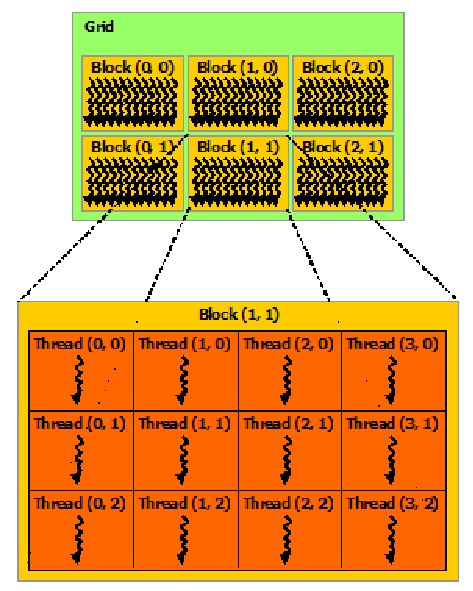
\includegraphics[width=\linewidth]{figs/threadBlock.pdf}
\caption{The thread/block hierarchy used in NVIDIA GPUs.
Image taken from Ref.~\cite{NVIDIA}.}
\label{fig:threadBlock}
\end{figure}


\section{Improving performance}

For pure $\SU(2)$ simulations like what I did in grad school, 
it may take months (or years!) for a single-processor MCMC simulation to
generate enough data to get reasonable error bars. In order to get
results in time to finish a PhD thesis, it is necessary to consider ways to
optimize the code.

When getting into details about coding specifically, this section tends to focus
on C++ and Python. Besides being two languages with which I'm comparatively
familiar, they are also popular choices for scientific computing. When GPU
parallelization is mentioned, we discuss NVIDIA, although alternatives like AMD
and Intel exist nowadays.

\subsection{Parallelization}

A common strategy is to divide the lattice into smaller sublattices, updating
simultaneously on each sublattice, passing relevant information between the
sublattices whenever necessary. {\it Parallelizing}\index{parallelization} 
in this way offers a speed
up factor somewhat less than the number of sublattices used. A standard way to
parallelize code is to use the Message Passing Interface (MPI). MPI\index{MPI} 
is a library that allows for efficient exchange of information between processors 
and can be included in Fortran, C, and C++ programs.

One way to approach parallelism is called Single Instruction Multiple
Data\index{SIMD} (SIMD). In this approach, the same instruction is given to
multiple data elements. For instance the first way you learn implement scalar
multiplication for a vector is through a simple loop:
\begin{verbatim}
do from i=0 to i=ndim
  v[i] *= 2
end do
\end{verbatim}
Instead of saying ``perform this multiplication, now perform the next one", SIMD
says to perform all the multiplications simultaneously, at least in the ideal
case. Sometimes this approach is referred to as {\it
vectorization}\index{vectorization}.

To get a quantitative understanding of performance, one introduces
the {\it clock cycle},\index{clock cycle} which is the smallest unit of
time in a computer\footnote{Most CPUs keep time using a quartz crystal.
The basic idea is that an electric field will cause the quartz to
vibrate. The frequency of this vibration is the clock cycle.
This frequency can be tuned according to the shape and size of the
crystal, as well the placement of electrodes on it.}.
In the olden days, only one computation would be carried out per cycle;
nowadays it is more common to carry out many. The number of
computations per clock cycle is known as the\index{clock speed} {\it clock speed}.

A CPU\index{CPU} is divided into several\index{core} physical {\it cores}, each of which can
carry operations separately. This is then one way to carry out parallelization:
You use MPI to have each core execute different tasks simultaneously.
A virtual entity comprising of these tasks being executed on one core
is usually called a\index{thread} {\it thread}. Sometimes one core splits
tasks between two threads. For pure $\SU(2)$ calculations, this
is sufficient.

We will see in \chref{ch:ferm} that simulations with dynamical fermions
are much more complex, and correspondingly, they are much more
computationally intensive. For such purposes, it is not really ideal even
to use CPUs. It was realized in the 2000s~\cite{egri_lattice_2007}
that\index{GPU} GPUs, which
are often needed for the numerous calculations required to render graphics
in video games, could be adapted for use in lattice QCD calculations.
In a GPU, there are many (often thousands) of cores, which allows for
extremely high parallelization. On a single GPU, no MPI is required;
however GPUs have memory limitations, such that they may not always accommodate
a single lattice, and in such cases MPI can be used to link
multiple GPUs together\footnote{How you link GPUs together depends on the
system you run on. Usually communication between GPUs is the slowest part
of a calculation, so one may utilize other frameworks besides MPI, usually
depending on the GPU manufacturer, to get a performance boost.}.
Since there are so many cores, it is practical to introduce an organizational
hierarchy. The most common is used by NVIDIA, where threads are collected
into\index{block} {\it blocks}; this is shown in \figref{fig:threadBlock}.

\subsection{Evaluating performance}

Lattice projects studying physically realistic setups
 are extremely computationally demanding; for instance
a recent HotQCD study utilized ensembles that required
$\order{2000}$ GPU-years of compute time and take up 2.4 PB of storage 
space~\cite{Bollweg:2021vqf}. Meeting these computational demands is
not cheap, and it is no longer sufficient to simply foist your
calculation onto GPUs. For these applications, it becomes crucially 
important that your code is highly
optimized to get the most bang for your buck.
We'll now review some key concepts and terminology
relevant to assessing the performance of code
in high-performance computing\index{high-performance computing} (HPC). 

In this context, it is useful to define a few terms. A floating
point operation\index{FLOP} is a calculation of floating point arithmetic. In a
scientific context, this type is very common, so FLOPs are a good indicator
of the amount of arithmetic a code is doing. Any scientific code you write will
be in effect processing data. The rate at which data is processed
is called the {\it throughput},\index{throughput} 
and it can be measured in, for instance, FLOPs
per second, sometimes indicated\footnote{Please take care not to
mix up FLOPs with FLOP/s.} FLOP/s. The rate at which data is
transferred is called the {\it bandwidth},\index{bandwidth}
which can be measured in bytes/s.

\begin{figure}[t]
  \centering
  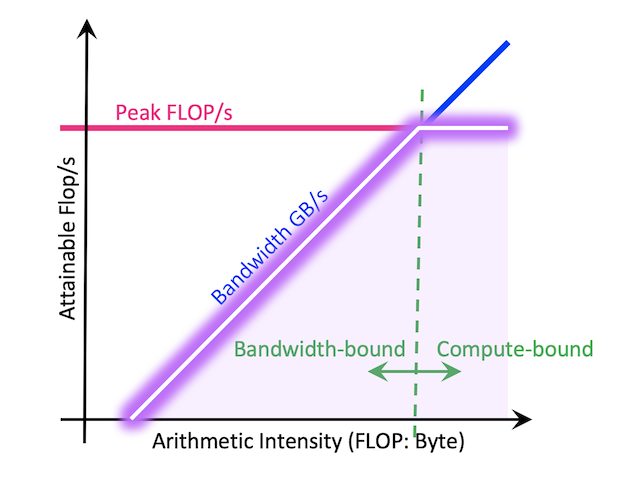
\includegraphics[width=\linewidth]{figs/Roofline-intro.png}
  \caption{Schematic example of a roofline analysis.
           Image taken from Ref.~\cite{roofline}.
           The light purple line indicates the theoretical
           maximum performance under this model.}
  \label{fig:roofline}
\end{figure}

\index{roofline performance analysis}
Obviously performance is limited by the hardware carrying out a calculation, for
instance the CPU, but it is also limited by the rate at which things are loaded
and extracted from memory. The {\it roofline performance model} is an elementary
way to see where your code stands with respect to these two limitations.

The {\it arithmetic intensity}\index{arithmetic intensity} of some code is
\begin{equation}
  \text{AI}=\frac{\text{\# FLOPs}}{\text{data movement in bytes}},
\end{equation}
where the numerator represents the number of FLOPs needed by that code, and the
denominator represents how much data you need to move in bytes in order to
support those FLOPs. From this equation it's clear that the attainable
FLOP/s scales linearly with arithmetic intensity.

Fig.~\ref{fig:roofline} shows a sketch of this model. The vertical
dashed line gives the {\it machine balance point}.\index{machine balance point}
This analysis is useful to try to diagnose whether one should look into
memory efficiency or algorithm improvement to try to speed up the code.
Code in the purple region to the left of the machine balance point
tends to be limited by bandwidth.

When it comes to evaluating the performance as one increases the number
of GPUs, a straightforward approach is to simply plot throughput against
the number of devices. In this context, one may be interested in
{\it strong scaling}\index{scaling!strong}, which measures the effectiveness 
of a parallel computing system when the problem size\footnote{In the context
of LQCD, the problem size is usually proportional to the lattice size
$N_\sigma^3\times N_\tau$.} remains constant, 
but the number of processing elements (cores, nodes, etc.) is increased.
In the ideal case\footnote{We never achieve the ideal case because of,
for instance, communication overhead.}, throughput
increases linearly with the number of processing elements.
One can also investigate {\it weak scaling}\index{scaling!weak},
which evaluates the performance when both the problem size and the number 
of processing elements are increased proportionally. 
Hence for a weak scaling test, the work assigned to each processing element 
remains fixed as new resources are added. Like with strong scaling,
perfect weak scaling would suggest throughput increases linearly with
the number of processing elements. In practice, it is much easier to
get closer to ideal weak scaling. There can be many reasons
for this, but a major one is that if the number of processors becomes
comparable to the number of computations, the code will spend a significant fraction
of the time communicating, which is hugely inefficient. Hence weak scaling is
usually a more relevant performance metric. 


\subsection{Optimizing memory usage}\label{sec:memory}

If you find your code is bandwidth-bound, there are a number of strategies that
can be used to improve performance. One way is to reshape your algorithm so that
it requires less communication. This can be quite challenging. An easier way is
to look in detail where your memory is being stored. Modern computing
architectures have multiple levels of memory, organized in the following by
increasing distance from the processor:
\begin{enumerate}
  \item {\it Registers}\index{register} are located inside of the processor
itself. They hold very little data but are extremely fast.
  \item {\it Caches}\index{cache} are also located inside the processor.
Actively used data from the main memory, which we'll discuss next, is duplicated
in the cache for faster access. A processor can contain a cache hierarchy, for
instance many GPUs have L1, L2, and L3 caches, which in that order become
gradually larger but slower.
  \item {\it Main memory}\index{memory!main} is no longer inside the processor,
but has a comparatively large storage size. It is connected to the processor
via a {\it bus}\index{bus}. On circuit boards, you can sometimes see the 
connections as thin lines of a metal, such as copper, called {\it
traces}\index{trace}. The bus also requires logical units made of transistors
that manage the this transfer between devices.
Usually there are multiple buses connecting the main
memory with the processor, for instance one bus may send a number that indicates
the desired location of the data. This number is the {\it memory address}.
Another bus will then transfer the data themselves.
\end{enumerate}
As already hinted in some of the above discussion, as one increases physical
distance from the processor, the latency tends to increase, or conversely the
bandwidth decreases. This increase in latency has many causes, the easiest of
which to understand are:
\begin{enumerate}
  \item Memory addresses correspond to physical locations on the storage device.
Reading and writing data is implemented through some physical operation at that
physical location, and hence you may lose time if you need to change locations,
depending on how this is implemented. Registers and caches let you carry out
repeated operations on a section of your full memory, limiting latency of this kind.
  \item Coordinating data transfer requires instructions to be sent around. The
further away the memory is, the more complicated it is to access that memory,
and hence the more instructions are required. And of course it takes time to
process instructions.
\end{enumerate}

\section{C++ best practices}

As discussed in the last section, achieving optimal performance is challenging
and subtle. When writing a lattice code, it is therefore crucial to choose
a language that
\begin{enumerate}
  \item gives the programmer control over technical details like how hardware
interactions are handled and how memory is stored; and
  \item allows the programmer to write code that is highly readable and
easy to use, so that the code can continue to be used and maintained
for a long time.
\end{enumerate}
These two requirements rule out almost every language except C++, which has
become the de facto standard for high-performance LQCD code\footnote{For
instance the two most widely-used code bases, Grid and QUDA, are both
written in C++. \simulat, which I work on, is also written in C++.}.
In the interest of point 2 above, it is worthwhile to discuss some
best practices in C++ programming.

When making new classes, one often has to think how memory should be allocated
and deallocated, in particular when defining constructors. The {\it rule of
three}\index{rule of three} states that whenever a type needs one of the
following, it needs all three:
\begin{itemize}
  \item copy constructor,
  \item copy assignment,
  \item destructor.
\end{itemize}
A common example where this is especially important is when your destructor 
explicitly deallocates some memory. If no user-defined copy constructor exists,
C++ implements a {\it shallow copy}\index{copy!shallow}. A shallow copy of an
object shares some of the same data as the original object, such as a 
pointer\footnote{By contrast, a {\it deep copy}\index{copy!deep} will create
an entirely new object with its own data.}.
Hence changing the attribute of a shallow copy will also change the attribute of
the original. This means that when the destructor is called on a shallow copy,
it will deallocate the original copy's data, and hence when it comes time for
the original copy to deallocate, there is nothing left!
This leads to {\it undefined behavior}\index{undefined behavior}, which is sort
of a catch-all term for a result of compiling and running that cannot be
predicted\footnote{When doing parallel computing, a commonly encountered type of
undefined behavior is a {\it race condition}\index{race condition}. 
This happens whenever two
processes try to write into the same chunk of memory at the same time. In my
experience, undefined behavior due to a race condition may not even produce the
same results after two runs of the same compilation.}. Compilers will not always
catch undefined behavior; hence it's safest to just use the rule of three from
the beginning.

An extension to the rule of three is the {\it rule of five}\index{rule of five},
which states that whenever a type needs one of the
following, it needs all five: 
\begin{itemize}
  \item copy constructor,
  \item copy assignment,
  \item destructor,
  \item move constructor,
  \item move assignment. 
\end{itemize}

A strategy to help improve code reuse and flexibility is\index{policy!based
design} {\it policy-based design}.
In this context, a {\it policy}\index{policy} is a template that encapsulates a 
behavior or set of behaviors that can be used to customize the behavior of a class. 
The policy itself is not part of the class, but rather is used to customize it. 
For example, a policy may determine how memory is allocated for an object
or how arithmetic with that object works.

The use of template parameters helps increase the flexibility of already
compiled code. In this context it is often to keep the
{\it substitution failure is not an error} (SFINAE)\index{SFINAE} principle
in mind.
SFINAE is a principle in C++ template metaprogramming that allows a template 
specialization to be discarded or selected based on whether a substitution 
failure occurs during template instantiation. This principle enables compile-time 
conditional behavior by selectively removing template specializations from 
consideration when certain conditions are not met.

\subsection{C++ referencing and dereferencing}

By default, if I pass an array to a function in C++, the function will get a
copy of the array, rather than the original. This is safe default behavior to
have; for example in a situation like
\begin{equation}
\text{output}=f(\text{input}),
\end{equation}
this precludes the possibility of modifying the original input array inside the
function by accident. On the other hand, this is inefficient: From the
discussion \secref{sec:memory}, you can imagine that copying an array then
accessing that copy may take some extra time. It obviously also takes up extra
memory, which is bad for extremely large arrays, like the ones that store gauge
fields.

The solution in C++ is to pass instead a {\it reference}\index{reference} to an 
array\footnote{Superficially pointers and references act similarly, but they are
different. A pointer contains a memory address, hence it takes up however much
memory is required to store that address. A reference is simply an alias, so it
takes up no memory.} as the argument. This can be accomplished with the
ampersand like
\begin{equation*}
\texttt{func(\&arr)}.
\end{equation*}
We say in the above case the function was ``passed by reference". In the
instance where we don't use reference, we ``pass by value" as
\begin{equation*}
\texttt{func(arr)},
\end{equation*}
which copies the array, as discussed above.

If we have a reference or pointer to some object in our code, we might be interested in
getting the value. This is accomplished through {\it
dereferencing}\index{dereference} by
\begin{equation*}
\texttt{value = *arr},
\end{equation*}
which would return the value of the first element of the array \texttt{arr}.

\subsection{C++ compile-time directives}

In the introduction of \secref{sec:oop}, I tried to distinguish between compile time
and run time. This is helpful for example to distinguish between information
that is known while compiling and known while running. In the context of lattice
QCD, it is beneficial to make the lattice size a run-time quantity. If it were a
compile-time quantity, then you would have to recompile your code each time you
changed lattice sizes.

Broadly speaking, when writing a code, one specifies a sequence of commands that
should be carried out. The role of the compiler is to translate those commands
to machine code, preferably in a safe away with good performance. C++ also gives
you the power to give commands to the compiler itself, i.e. you can control to
some degree how the compiler translates the code. For example a compile-time
decision might be whether to compile in single or double precision. One can
specify which decision to make using a {\it compile-time
directive}\index{compile time!directive}.
In C++ these are usually indicated with the \texttt{\#} symbol.

A series of such directives can be used to simplify coding tasks or create
coding shortcuts. In this context sometimes one refers to such series as {\it
macros}\index{macro}.

\bibliographystyle{unsrtnat}
\bibliography{bibliography}
